\chapter{Glavna ploča}
\label{pog:mainboard}

Sustav se sastoji od dva uređaja koji rade u simbiozi. Glavna ploča služi za snimanje, obradu i pohranu glasovnih podataka i obradu i pohranu biomedicinskih parametara. Za snimanje biomedicinskih parametara koristi se narukvica. U ovom poglavlju se opisuje glavna ploča.

Zahtjevi na glavnu ploču su sljedeći:
\begin{itemize}
    \item mikrokontroler \engl{Microcontroler Unit, MCU}, dovoljno moćan za pokretanje neuralnih mreža i obradu podataka
    \item konektor za SD karticu
    \item bežična komunikacija putem Wi-Fi ili Bluetooth sučelja
    \item praćenje vremena putem RTC-a
    \item mikrofon za prikupljanje govora korisnika
    \item sučelja za testiranje i prženje koda na mikrokontroler
    \item napajanje i punjenje baterije preko USB C priključka
    \item baterijsko napajanje putem litij-ionske baterije
\end{itemize}
U daljnjem tekstu ovog poglavlja opisane su odabrane komponente, kao i razlog njihova odabira, način, razlozi i proračuni dizajna pojedinih podsustava, te dizajn, proizvodnja i testiranje PCB-a.

\section{Mikrokontroler}
Za mikrokontroler odabran je STM32F746VG baziran na Cortex-M7 arhitekturi koji integrira funkcionalnosti digitalne obrade signala, bogat sa svim potrebnim periferijama za integriranje s ostatkom sustava i dovoljno procesorske snage za obavljanje zadanog zadatka. Također, programska potpora je razvijena na razvojnom sustavu BLABLABLA, pa je ovaj mikrokontroler odabran radi lakšeg razvoja cjelokupnog sustava. Shema napajanja mikrokontrolera prikazana je na slici \ref{slk:MCU_PS}, a shema spajanja mikrokontrolera s ostatkom sustava prikazana je na slici \ref{slk:MCU_PE}.

\begin{figure}[hbt]
    \centering
    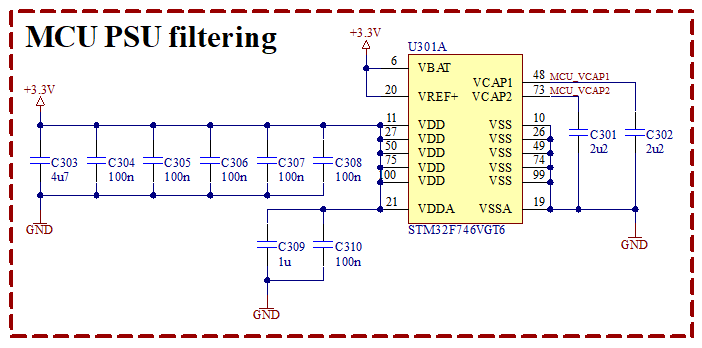
\includegraphics[width=\textwidth]{Figures/MCU_02.png}
    \caption{Shema napajanja mikrokontrolera}
    \label{slk:MCU_PS}
\end{figure}

Shema napajanja napravljena je prema uputama proizvođača \cite{stmicroelectronics:an4661}. S obzirom na to da na ovoj ploči nema analognih signala, nije potrebno raditi analogno-digitalnu pretvorbu, pa su stezaljke za napajanje analognog dijela mikrokontrolera spojene sa stezaljkama za napajanje digitalnog dijela. Također, nije potrebna precizna naponska referenca, a baterijskim napajanjem će upravljati vanjski čip, pa su te dvije stezaljke spojene na napajanje od +3.3 V.
\newpage

\begin{figure}[hbt]
    \centering
    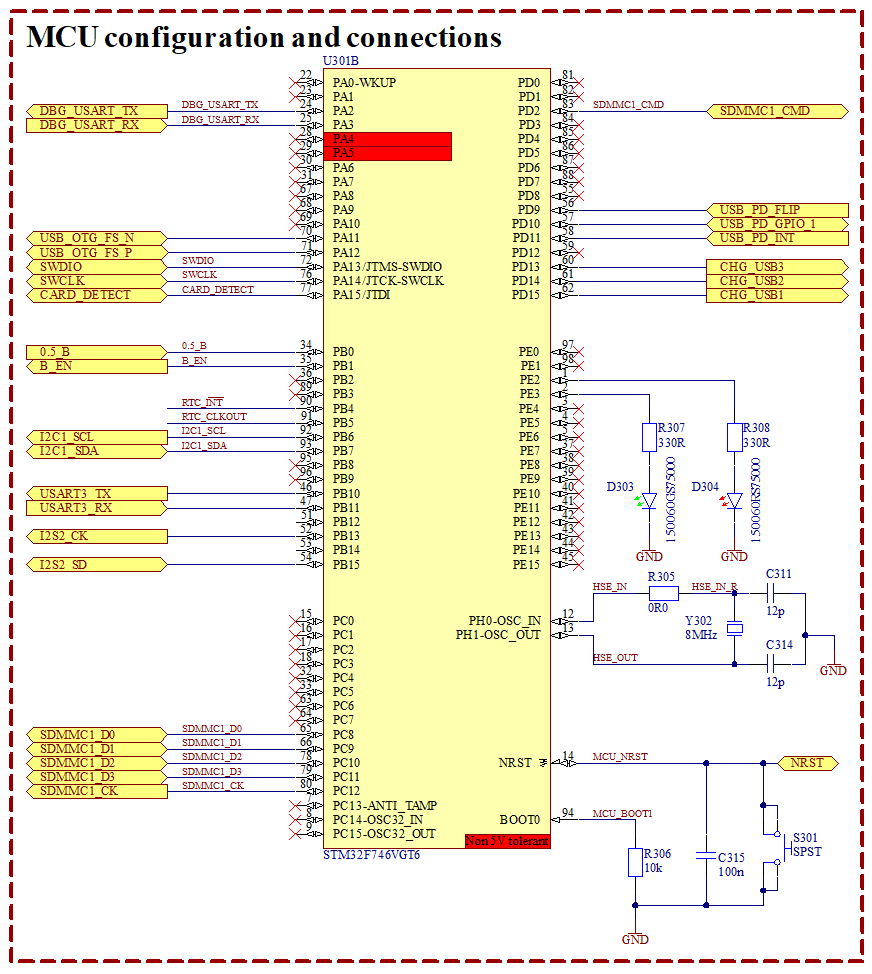
\includegraphics[width=\textwidth]{Figures/MCU_01.png}
    \caption{Shema periferije mikrokontrolera}
    \label{slk:MCU_PE}
\end{figure}

Postavljene su dvije svjetleće diode za pomoć pri programiranju i tipka za reset mikrokontrolera. Kod određivanja korištenih stezaljki za pomoć je korišteno razvojno okruženje STM32CubeIDE. Dizajn oscilatora opisan je u priručniku proizvođača STMicroelectronics \cite{stmicroelectronics:an2867}. Oscilator koji mikrokontroler koristi je Pierceov oscilator (slika \ref{slk:PIERCE}).
\begin{figure}[hbt]
    \centering
    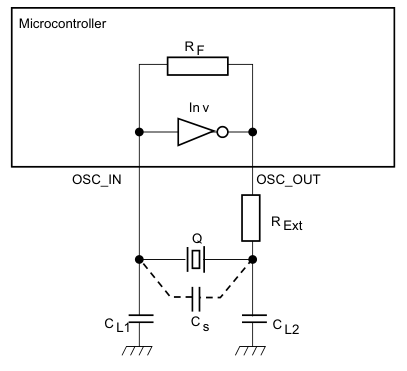
\includegraphics[width=10cm]{Figures/pierce.PNG}
    \caption{Shema Piercovog oscilatora \cite{stmicroelectronics:an2867}}
    \label{slk:PIERCE}
\end{figure}

\subsection{Pierceov oscilator}
Pierceov oscilator se sastoji od invertera \textit{Inv}, koji radi kao pojačalo, kristala \textit{Q}, otpornika u povratnoj vezi \textit{R\textsubscript{F}}, vanjskog otpornika za ograničenje izlazne struje invertera \textit{R\textsubscript{Ext}}, vanjskih kapaciteta opterećenja \textit{C\textsubscript{L1}} i \textit{C\textsubscript{L2}}, parazitskog kapaciteta PCB-a i kapaciteta između stezaljki mikrokontrolera \textit{C\textsubscript{s}}.

Uloga otpornika \textit{R\textsubscript{F}} je da natjera inverter da se ponaša poput pojačala. Otpornik povratne veze je spojen između izlaza i ulaza pojačala čime se ulaz i izlaz drže na istom naponi i prisiljava pojačalo da radi u linearnom području rada. Ovaj otpornik je integriran u mikrokontroleru zajedno s pojačalom.

Kapacitet opterećenja je ukupni kapacitet povratne veze oscilatora i mora biti jednak je kapacitetu između stezaljki kristala kako bi oscilator prooscilirao. Kapacitet opterećenja specificira proizvođač kristala i označava se s \textit{C\textsubscript{L}}. Vanjskim kondenzatorima \textit{C\textsubscript{L1}} i \textit{C\textsubscript{L2}} se postavlja kapacitet opterećenja povratne veze kako bi odgovarao kapacitetu opterećenja kristala. Kapacitet opterećenja računa se prema sljedećoj jednadžbi:
\begin{equation} \label{eq:CLOAD}
    C_L=\frac{C_{L1}\cdot C_{L2}}{C_{L1}+C_{L2}}+C_s
\end{equation}

Kod dizajna oscilatora potrebno je izračunati kritično pojačanje petlje:
\begin{equation} \label{eq:GMCRIT}
    g_{mcrit}=4\cdot ESR \cdot {(2\pi F)}^2\cdot {(C_0 + C_L)}^2
\end{equation}
gdje je \textit{F} frekvencija oscilatora, \textit{ESR} serijski otpor kristala i \textit{C\textsubscript{0}} serijski kapacitet kristala. Ovaj parametar je potrebno izračunati kako bi se moglo provjeriti hoće li se oscilator upaliti i prooscilirati. Dobiveni podatak se uspoređuje sa specificiranim vrijednostima transkonduktivnosti \textit{g\textsubscript{m}} u dokumentaciji mikrokontrolera. Da bi oscilator proradio mora se proračunati margina pojačanja i treba vrijediti:
\begin{equation} \label{eq:GMARGIN}
    {gain}_{margin}=\frac{g_m}{g_{mcrit}}>5
\end{equation}

Kako ne bi došlo do kvara kristala potrebno je ograničiti snagu koja se na njemu disipira s pomoću vanjskog otpornika \textit{R\textsubscript{Ext}}. Maksimalna snaga koja se može disipirati na kristalu naznačena je u dokumentaciji proizvođača. Ovaj otpornik s kondenzatorom \textit{C\textsubscript{L2}} formira niskopropusni filtar kako bi oscilator proradio na osnovnoj frekvenciji, a ne na višim harmonicima. Ako snaga disipirana na kristalu bude veća od maksimalne dozvoljene onda je vanjski otpornik obavezan i mora se proračunati, u suprotnom ga nije potrebno stavljati. Vrijednost otpornika se računa na sljedeći način:
\begin{equation} \label{eq:REXT}
    R_{Ext}=\frac{1}{2\pi F C_{L2}}
\end{equation}

\subsection{Dizajn oscilatora}

Oscilator je vidljiv na slici \ref{slk:MCU_PE}. Odabran je kristal NX8045GB proizvođača NDK. Njegove karakteristike su sljedeće:
\begin{itemize}
    \item \textit{C\textsubscript{L}} = 2 pF
    \item \textit{ESR} = 200 $\Omega$
    \item \textit{F} = 8 MHz
\end{itemize}
\textit{C\textsubscript{0}} nije naznačen pa se uzima vrijednost 0. Uzimajući za parazitni kapacitet \textit{C\textsubscript{s}} = 2 pF, i koristeći formulu \ref{eq:CLOAD} dobiju se vrijednosti kondenzatora \textit{C\textsubscript{L1}} = \textit{C\textsubscript{L2}} = 12 pF. Odabir parazitnog kapaciteta je odokativan jer se ne može znati unaprijed bez mjerenja dovršene tiskane pločice. Kod odabira kondenzatora potrebno je obratiti pažnju na dielektrik kondenzatora i tolerancije. Kako bi frekvencija oscilatora bila što stabilnija potrebno je koristiti temperaturno stabilan dielektrik, odnosno kondenzatore klase 1. Korišteni kondenzatori imaju C0G dielektrik. Koristeći jednadžbu \ref{eq:GMCRIT} dobiva se \textit{g\textsubscript{mcrit}} = 0.1294 mA/V. Iz dokumentacije mikrokontrolera se dobiva \textit{g\textsubscript{m}} = 1 mA/V. Iz uvjeta \ref{eq:GMARGIN} dobiva se \textit{gain\textsubscript{margin}} = 7.73, čime je uvjet zadovoljen. S obzirom na to da nije moguće odrediti koliko će se kristal grijati, za vanjski otpornik postavljen je otpornik vrijednosti 0 $\Omega$, pa u slučaju prevelike disipacije snage na kristalu moguće je na njegovo mjesto zalemiti otpornik odgovarajuće vrijednosti prema jednadžbi \ref{eq:REXT}.

